\documentclass{beamer}
\usepackage[utf8x]{inputenc}
\usepackage{ucs}
\usepackage{amsmath,tabularx}
\usetheme{CambridgeUS}
% \usecolortheme{crane}
% \usefonttheme{structurebold}
\newcolumntype{C}{>{\centering\arraybackslash}X}
\linespread{1.5}

\usepackage{subfigure}
\title[Hidden Structure]{\sc{ Combining latent topics with document attributes in text analysis}}
\author[NA]{Nelson Auner\\Advisors: Prof. Matt Taddy \& Prof. Stephen Stigler}

\institute[UChicago]{University of Chicago}
\date[13.05.2014]{May 13, 2014}

\usepackage{amsmath,supertabular,tabularx,graphicx,amssymb,amsfonts}
\usepackage{natbib,rotating}
%\usepackage{default}
\newcolumntype{Z}{>{\centering\arraybackslash}X}%



\renewcommand{\t}{\ensuremath{\theta}}
\renewcommand{\a}{\ensuremath{\alpha}}
\renewcommand{\b}{\ensuremath{\beta}}
\newcommand{\g}{\ensuremath{\gamma}}
\newcommand{\E}{\mathsf{E}}
\renewcommand{\d}{\ensuremath{\delta}}
\newcommand{\e}{\ensuremath{\epsilon}}
\newcommand{\s}{\sigma}
% \renewcommand{\S}{\Sigma}
\newcommand{\from}{\ensuremath{\leftarrow}}
\newcommand{\bm}{\mathbf}
\renewcommand{\l}{\lambda}
\newcommand{\dint}{\int\displaylimits}
\newcommand{\bx}{\mathbf x}
\newcommand{\by}{\mathbf y}
\newcommand{\be}{\pmb\e}
\renewcommand{\k}{\kappa}
\newcommand{\m}{\mu}
\newcommand{\A}{\ensuremath{\mathcal{A}}}
\newcommand{\B}{\ensuremath{\mathcal{B}}}
\newcommand{\sT}{\mathrm{T}}
\newcommand{\diag}{\mathrm{diag}}
\newcommand{\Tr}{\mathrm{Tr}}
\newcommand{\cov}{\mathbb{C}\mathrm{ov}~}
\newcommand{\var}{\mathbb{V}\mathrm{ar}~}


\AtBeginSection[]  % "Beamer, do the following at the start of every section"
{
\begin{frame}<beamer> 
\frametitle{Outline} % make a frame titled "Outline"
\tableofcontents[currentsection]  % show TOC and highlight current section
\end{frame}
}



\begin{document}
\begin{frame}<handout:0>
  \titlepage
\end{frame}

%%%%%%%%%%%%%%%%%%%

%\section{Text as Data }
%\subsection{Text}
%\subsection[Basic Structure]{Multinomial Models}
%\subsection{Metadata and Topic Models}
%\section{Cluster Membership Model}
%\subsection{Specification}
%\subsection[Parameter Estimation]{Estimation of Parameters}
%\subsection[Initialization]{Initialization of Cluster Membership
%\section{Application & Comparison with IRTM}
%\subsection{Congression Data}
%\subsection{Restaurant Reviews}
%\section{Extensions}
%\section*{References}


\section{Text as Data }
\begin{frame}
 \frametitle{Text as Data}
 \begin{itemize}
\pause
\item A document is a collection of phrases. 
\pause
\item Our datasets are collections of documents
\end{itemize}
\pause
\begin{table}[!hbpt]
\caption{What did homework consist of?} \label{tab:title}
\pause
\begin{center}
\begin{tabular} {c c}
\textbf{Document} & \textbf{Content} \\
\hline
1 & Some computation and formula proving, a lot of R code \\
2 & Problems, computation using R \\
3 & Some computations and writing R code\\
4 & Proofs, problems, and programming work \\
\end{tabular}
\end{center}
\end{table}
\end{frame}

\subsection[Basic Structure]{Multinomial Models}
\begin{frame}
\pause
\frametitle{Multinomial Models}
\begin{itemize}
\item If order doesn't matter, then we can treat each document as a "bag of words". 
\pause
\item The number of words can be modeled as a multinomial 
\pause
\end{itemize}
\begin{table}[!hbpt]
\caption{Creating a word-count matrix from text}
\begin{center}
\resizebox{\textwidth}{!}{%
\begin{tabular}{ c |  c c c c c c c c c c c}
\hline
\textbf{Document} & Some & comp & formula & prov & R & code & use &
problem & writ & program & work \\
1 & 1 & 1 & 1 & 1 & 1 & 1 & 0 & 0 & 0 & 0 & 0 \\
2 & 0 & 1 & 0 & 0 & 1 & 0 & 1 & 1 & 0 & 0 & 0 \\
3 & 1 & 1 & 0 & 0 & 1 & 0 & 0 & 0 & 1 & 0 & 0\\
4 & 0 & 0 & 0 & 1 & 0 & 0 & 0 & 1 & 0 & 1 & 1\\
\hline
\end{tabular}}
\end{center}
\end{table} 
\pause
\end{frame}


\begin{frame}
\frametitle{A better model: Metadata}
\begin{itemize}
\item We would like to add structure to the model for inference or prediction
\pause
\item Metadata is data that accompanies a document
\pause
\end{itemize}
\begin{table}[!hbpt]
\caption{What did homework consist of?} \label{tab:title}
\pause
\begin{center}
\begin{tabular} {l l}
\textbf{Grade} & \textbf{Content} \\
\hline
A+ & Some computation and formula proving, a lot of R code \\
B & Problems, computation using R \\
B & Some computations and writing R code\\
C+ & Proofs, problems, and programming work \\  %something about R :P
\end{tabular}
\end{center}
\end{table}
\end{frame}



\subsection{Metadata and Computation}
\begin{frame}
\frametitle{Metadata and Computation}
\begin{itemize}
\item $n$ documents with metadata that takes $m$ discrete values:
\item Normally, $n >> m$
\item $\Rightarrow$ "Collapse" by outcome variables. 
\item Model as $m$ observations, instead of $n$
\end{itemize}
\begin{table}[!hbpt]
\begin{center}
\resizebox{\textwidth}{!}{%
\begin{tabular}{ l |  c c c c c c c c c c c}
\hline
\textbf{Document} & Some & comp & formula & prov & R & code & use &
problem & writ & program & work \\
A+ & 1 & 1 & 1 & 1 & 1 & 1 & 0 & 0 & 0 & 0 & 0 \\
B & 1 & 2 & 0 & 0 & 2 & 0 & 1 & 1 & 1 & 0 & 0 \\
C & 0 & 0 & 0 & 1 & 0 & 0 & 0 & 1 & 0 & 1 & 1\\
\hline
\end{tabular}}
\end{center}
\end{table} 
\pause
Reality: There are thousands of course reviews
\end{frame}


\subsection{Topic Models}
\begin{frame}
 \frametitle{Topic Models}
In a topic model, documents are the realizations of mixtures of topics. \\ A topic is a distribution of words. 

\begin{columns}
\column{.3\textwidth}
\begin{block}<3->{Running Topic}
Stride, Pacing, Stretch
\end{block}
\column{.3\textwidth}
\begin{block}<2->{Bike Topic}
Pedal, Helmet, Gears
\end{block}
\column{.3\textwidth}
\begin{block}<4->{Swimming}
Stroke, Air, Water
\end{block}
\end{columns}
\begin{itemize}
A book about triathalon training $\sim$ Running + Biking + Swimming
\end{itemize}
\end{frame}



\begin{frame}
 \frametitle{What are we talking about?}
%  \begin{block}
 \begin{itemize}
  \item T--cells are a type of lymphocyte that play a central role in cell-mediated immunity. \alert{T cells are GOOD CELLS}.
  \item A T cell receptor or \alert {TCR} is a molecule that is found on T--cells.
  \item TCR recognizes antigens.
  \item Thus TCR is linked with the immunity system of a mammal (contrary to the T--virus which create zombies).
  \end{itemize}
%    \end{block}
\end{frame}

\begin{frame}
\frametitle{Types of T--cells}
 \begin{center}
  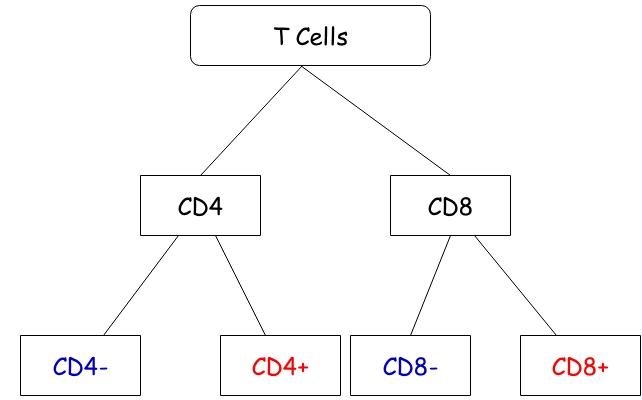
\includegraphics[width=0.8\textwidth]{TCELLS}
 \end{center}
\end{frame}

\end{document}

